\begin{figure}[t]
\centering\small
\begin{subfigure}[t]{0.32\linewidth}
  \centering
  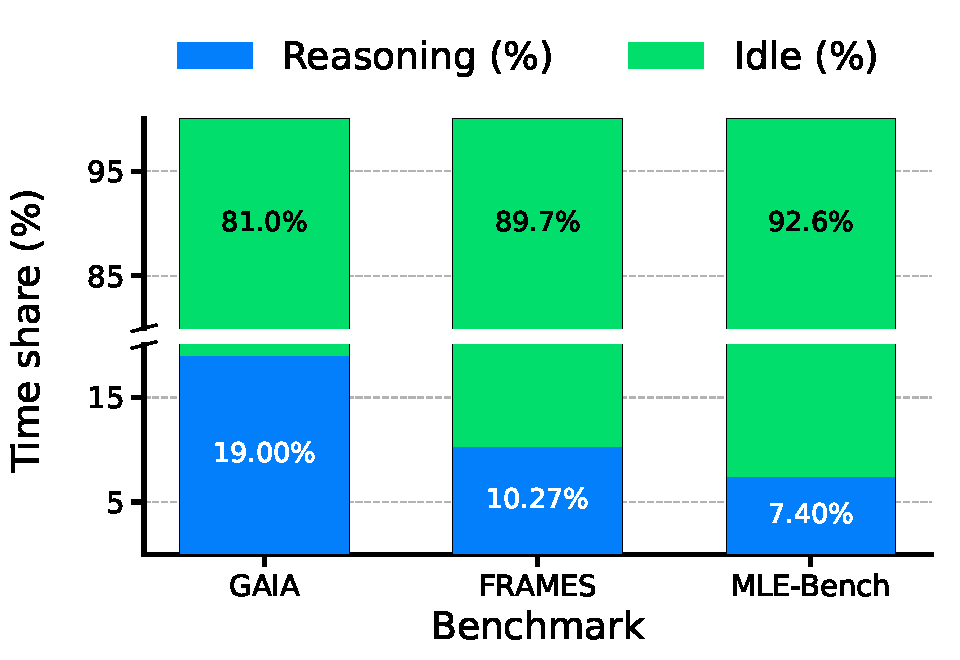
\includegraphics[width=\linewidth]{figures/observation_source_new.pdf}
  \caption{Idle vs.\ Reasoning Share}
  \label{fig:observation-source}
\end{subfigure}\hfill
\begin{subfigure}[t]{0.32\linewidth}
  \centering
  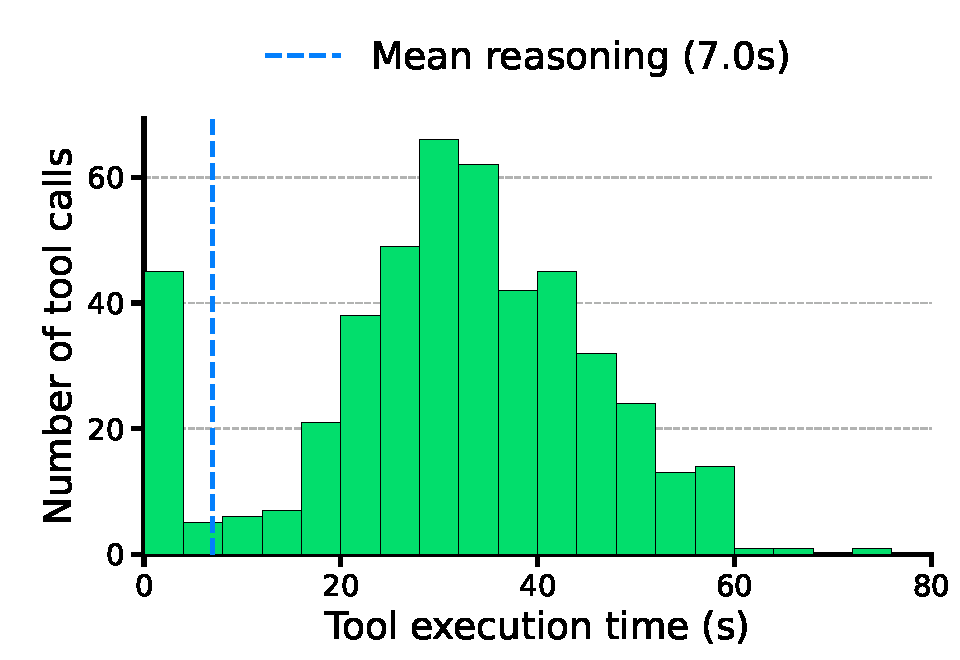
\includegraphics[width=\linewidth]{figures/observation_tool_execution_time_new.pdf}
  \caption{Tool Execution Time}
  \label{fig:observation-tool-execution-time}
\end{subfigure}\hfill
\begin{subfigure}[t]{0.32\linewidth}
  \centering
  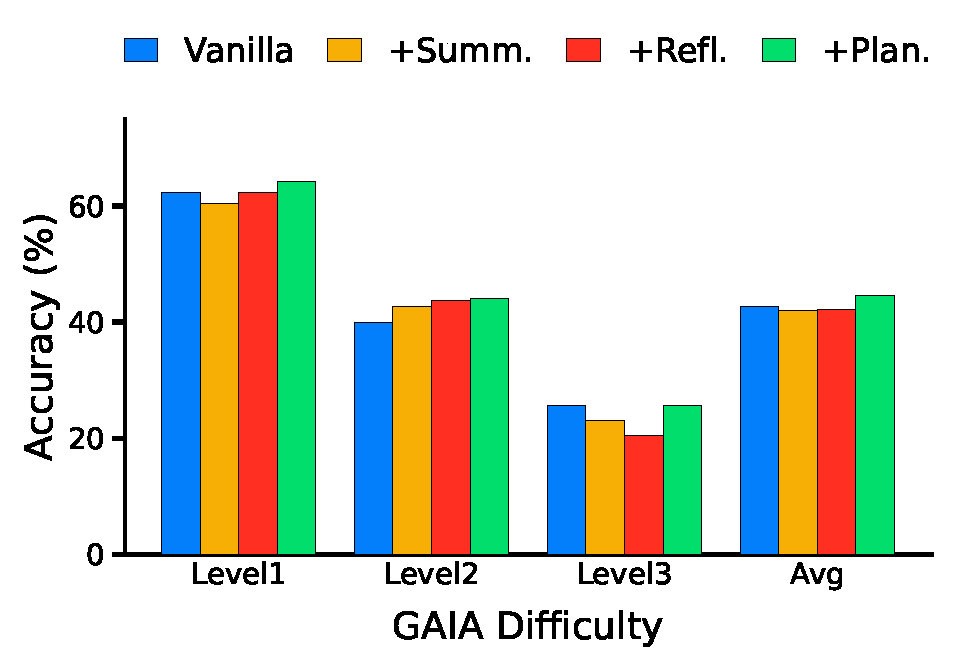
\includegraphics[width=\linewidth]{figures/observation_methods.pdf}
  \caption{Idle-Time Strategies}
  \label{fig:observation-methods}
\end{subfigure}
\caption{\textbf{How Can We Leverage Idle Time in LLM Agents?}
(a) Reasoning time vs.\ tool execution time (\ie idle time) across benchmarks.
(b) Histogram of per-call tool execution times. 
(c) Accuracy of three idle-time strategies (Summarization, Reflection, Planning) vs.\ vanilla.}
\label{fig:observation-idle}
\end{figure}

\section{How Can We Leverage Idle Time in LLM Agents?}\label{sec:observation}
In this section, we investigate the following key questions: how much reasoning budget is available during idle time, and which strategies are effective for utilizing it. To this end, we conduct experiments on 
three benchmarks:
(i) GAIA, in which agents invoke diverse external tools such as web 
search, file readers, and multimodal parsers;
(ii) FRAMES, which contains multi-hop questions requiring long chain
of sequential search-based tool calls; and
(iii) MLE-Bench, which involves ML workloads (model training, 
evaluation) that produce substantial environment response delays.

\subsection{Source of Idle Time}
To quantify the reasoning budget available during idle time, we visualize
the ratio of tool execution to reasoning time. As shown in
Figure~\ref{fig:observation-source}, tool execution
dominates the total execution time (e.g., it is more than 12.5x larger
than reasoning time in MLE-Bench), leaving a substantial reasoning budget
unused.
Beyond this aggregate gap, the per-call statistics in Figure~\ref{fig:observation-tool-execution-time} reveal that idle durations are highly heterogeneous within a single trajectory, ranging from shorter than a single reasoning step (the dashed line) to more than 10x longer. The long tail of this distribution accounts for the majority of total idle time and is large enough to support \emph{multiple} rounds of speculative computation, making it the opportunity for idle-time exploitation.

\subsection{Strategies for Idle Time}\label{subsec:obs2}
To identify effective idle-time strategies, we compare three representatives against a vanilla baseline without idle-time computation:
(i) \textit{summarization}, which compresses the interaction history;
(ii) \textit{reflection}, which evaluates the current action based on past trajectories; and
(iii) \textit{planning}, which generates candidate plans conditioned on plausible future observations.
As shown in Figure~\ref{fig:observation-methods}, only planning consistently matches or exceeds the baseline across all difficulty levels, achieving the highest average accuracy, while summarization and reflection fail to deliver consistent gains and even degrade performance (e.g., a notable accuracy drop for reflection on GAIA Level 3).
We attribute this to differences in how each method handles observation uncertainty during idle time. Summarization and reflection must commit to an incomplete interpretation of the trajectory before future observations arrive (e.g., reflection misjudging a valid action as erroneous), which then propagates into subsequent decisions. Planning avoids this by admitting a conditional formulation over possible future observations (e.g., if A holds, execute X; otherwise Y), making idle-time compute resilient to this uncertainty.
